\chapter{Introduction}
\label{ch:Introduction}

\paragraph{ }The aim of technology review is to understand the working of all the tools and observing pros and cons of the technologies relevant to this project.

To achieve this, tasks were assigned to each of the team to review set of tools as below. 

\begin{figure} [h]
\centering
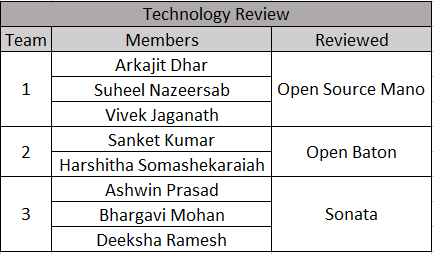
\includegraphics[width=.5\linewidth]{figures/teams}
\end{figure}

MANO frameworks such as Open Source MANO, Sonata and Open Baton have been reviewed in this phase. Different Virtual Infrastructure Managers(VIM) Experimented like Open Stack and Kubernetes.\\*

The MANO frameworks are up and running in virtual machines and the connections are established between MANO and VIM.\\*

The detailed explanation on installation steps are given below in the document. Conclusion of the technology review includes the possible features that could be added.



